\subsection{Korrelation der X- und Y-Histogramme (Jan)}

Für die Korrelation der X- und Y-Histogramme haben wir denselben Ansatz wie auch schon für die Korrelation der Winkelhistogramme verfolgt. Das X- bzw Y-Histogramm des neuen Scans wird gegen das X- bzw. Y-Histogramm des alten Scans verschoben und eine X- bzw. Y-Korrelation wird für alle Verschiebungen berechnet. Am linken Rand der Korrelation befindet sich der Wert für eine Verschiebung um 0. Nach rechts ist dann eine positive Verschiebung aufgetragen. Die Verschiebung ist zyklisch geschlossen, deshalb ist eine große positive Verschiebung gleichbedeutend mit einer kleinen negativen Verschiebung.

\begin{figure}
	\centering
	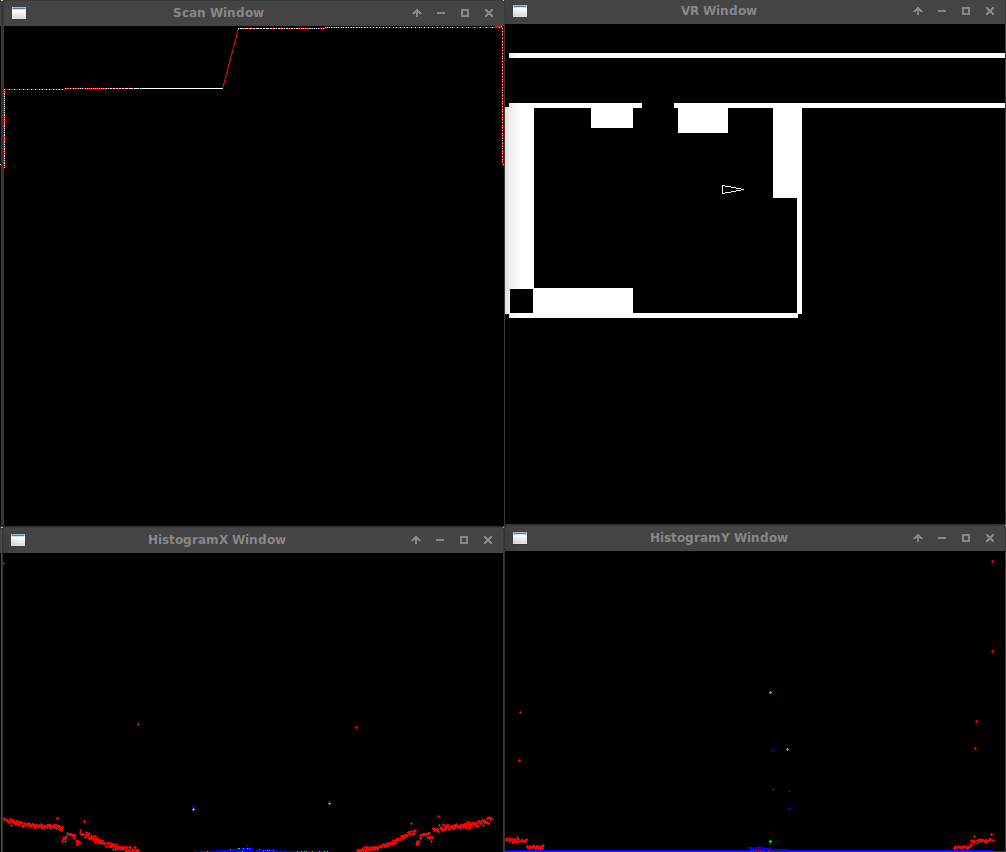
\includegraphics[width=16cm]{XYhistogram_neu}
	\caption{Oben links befindet sich der aktuelle Scan, oben rechts eine Darstellung des Roboters im virtuellen Raum, unten befinden sich die X- und Y-Histogramme einer Bewegung in Y-Richtung auf eine Wand zu. In blau ist das Histogramm des alten Scans eingetragen, in grün das Histogramm des neuen Scans und in rot die Korrelation der beiden Scans}
	\label{fig:xyhistogram}
\end{figure}

Abbildung~\ref{fig:xyhistogram} stellt die Histogramme und deren Korrelation bei einer Bewegung des Roboters in Y-Richtung auf eine Wand zu dar. Im X-Histogramm lässt sich deutlich erkennen, dass der Roboter sich parallel zu den Wänden bewegt. Die Maxima der neuen und alten Korrelation liegen fast genau aufeinander. Dadurch liefert auch die Korrelation ein Maximum bei einer Verschiebung um 0. Im Y-Histogramm lässt sich erkennen, dass sich vor dem Roboter zwei Wände befinden, eine etwas weiter entfernt als die andere. Die grünen Punkte befinden sich etwas näher am Roboter als die blauen Punkte, der Roboter fährt also auf die Wände zu. Dies wird auch durch die Korrelation gezeigt, die ein Maximum bei einer ganz leicht negativen Verschiebung zeigt. Dass die blauen Maxima kleiner sind als die grünen Maxima, ist dem Umstand geschuldet, dass die Wand sich im alten Histogramm auf mehrere Bins des Histogramms aufteilt, weil sie genau auf einem Übergang liegt.